\documentclass[msc]{ppgccufmg}
\usepackage[english]{babel} % english | brazil
\usepackage[utf8x]{inputenc}
\usepackage[T1]{fontenc}
\usepackage{type1ec}
\usepackage{graphicx}
\usepackage[a4paper,
  portuguese,
  bookmarks=true,
  bookmarksnumbered=true,
  linktocpage,
  colorlinks, 
  citecolor=black,
  urlcolor=black,
  linkcolor=black,
  filecolor=black,
  ]{hyperref}
\usepackage[square]{natbib} %,numbers

% Additional Packages (Ueda)
\usepackage{tabularx}
\usepackage{scalerel}
\usepackage[dvipsnames]{xcolor}
\usepackage{nameref} % For cross-refering section titles
\usepackage{amsmath}
\usepackage{amssymb}
\usepackage{lmodern} % Cool font

\include{definitions}

% Portuguese hyphenation causing problems in the english text
\hyphenation{re-qui-si-to}

\begin{document}

% O comando a seguir, \ppgccufmg, provê todas as informações relevantes para a
% classe ppgccufmg. Por favor, consulte a documentação para a descrição de
% cada chave.
\ppgccufmg{
  title={Reputation in Computer Science\\ 
  	on a per Subarea Basis},
  authorrev={Ueda, Alberto Hideki},
  %cutter={D1234p},
  %cdu={519.6*82.10},
  university={Federal University of Minas Gerais},
  course={Computer Science},
  %portuguesetitle={Reputação em Ciência da Computação sob uma Perspectiva de Sub-Áreas},
  portugueseuniversity={Universidade Federal de Minas Gerais},
  portuguesecourse={Ciência da Computação},
  address={Belo Horizonte},
  date={2017-06},
  advisor={Berthier Ribeiro-Neto},
  coadvisor={Nivio Ziviani},
  abstract={Resumo}{resumo},
  abstract=[english]{Abstract}{abstract},
%  dedication={dedication},
%  ack={acknowledgements},   
%  epigraphtext={And again when it shall be thy wish to end this play at night,\\
%			I shall melt and vanish away in the dark,\\
%			or it may be in a smile of the white morning,\\
%			in a coolness of purity transparent.}
%			{Rabindranath Tagore},%, Bengali poet}
%  epigraphtext={- Arrogance and fear still keep you from learning \\ 
%  		the simplest and most significant lesson of all. \\
%        - Which is?\\
%        - It's not about you.}{Doctor Strange movie, 2016},
  indexkeys={1.~Computação --- Teses. 2.~Redes --- Teses. I.~Orientador.
    II.~Título.},
}

%%%%%%%%%%%%%%%%%%%%%%%%%%%%%%%%%%%%%%%%%%
\chapter{Introduction}
%%%%%%%%%%%%%%%%%%%%%%%%%%%%%%%%%%%%%%%%%%

Funding agencies, university officials, and department chairs constantly face the challenge of understanding how well the researchers they employ or sponsor are doing in terms of academic productivity and scientific impact. The assessment of their research quality usually includes the use of quantitative measures (e.g. citation counts, H-index) and/or qualitative surveys within their scientific community. For instance, in the US, the National Research Council (NRC) applied in 2010 an extensive survey to gather information about more than one hundred US graduate programs. 

Overall, such assessments aim to capture the \textit{reputation} of each scholar or the graduate program. That is, the perception of the researcher (or group of researchers) before the general public or before its/their academic peers. In principle, the researchers with high reputation should receive priority treatment in the allocation of grants, research funds, scientific awards, graduate students than less reputable researchers within the same community.

However, even the aforementioned NRC attempt to present an evidence-based ranking of US graduate programs has not been accepted without controversy \citep{vardi17}. Additionally, allocating research funds with basis on an unidimensional ranking of graduate programs in a given area ignores the complex interplay between individual traits and program's unique patterns of strengths and weaknesses. While private organizations are also able to produce such rankings, it has been argued that in this way third-party business interests may influence academic values \citep{brembs13}.

In this dissertation, we provide a complementary method for assessing reputation of publication venues and graduate programs on a per subarea basis. For that, we rely on a reputation metric previously introduced in the literature \citep{ribas2015random} and modify it to the context of subareas. We apply this novel metric to rank conferences, journals, and graduate programs in Computer Science (CS) in Brazil and US.

%%%%%%%%%%%%%%%%%%%%%
\section{Motivation}
%%%%%%%%%%%%%%%%%%%%%

The decision of which researchers should be at the top -- for hiring, promoting, funding, or distributing grants, scholarships, awards and so on -- is typically based on criteria such as number of publications, impact of publications, number of undergraduate and graduate students under supervision, number of advised MSc and PhD theses, and participation in committees (conferences, journal editorial boards, technical committees, etc). 
%
Therefore, the effectiveness of the resulting ranking depends on how each criterion is assessed and the period of time covered in the assessment. Several indices have become widely used to measure the productivity of researchers. Examples include the raw number of citations, h-index ~\citep{hirsch2005}, g-index \citep{egghe2006theory} and citation z-score \citep{zscore}. Likewise, most academic search platforms, such as Google Scholar\footnote{\url{http://scholar.google.com}}, Microsoft Academic Search\footnote{\url{http://academic.research.microsoft.com}} and ArnetMiner\footnote{\url{http://arnetminer.org}}, use some of such indices to rank researchers.

However, ranking researchers without regarding the specificity of their subareas or sub-fields of research is arguably unfair and potentially error-prone \citep{lima2013jcdl}. For instance, consider the problem of comparing the research output of two different researchers, where the first one works on a subarea $A$ and the second one works on a subarea $B$. If we assume that it is inherently harder to publish articles in $A$ than in $B$, it seems natural that the metrics used to rank these researchers should be distinct, or, at least, take those differences between subareas into account. Otherwise, the comparison between them would be unfair.

As an illustration, consider the subarea of Human-Computer Interaction within the broad field of CS. Experimental evaluation in this area usually takes more time than in other CS subareas when arranging and assessing users' feedback is necessary. On the other hand, CS subareas such as Databases and Computer Graphics do not usually face the same problem because their experimental evaluations depend on assessing the outcome of an automatic process, such as a query evaluation or a graphics rendering engine. Likewise, researchers from some subareas may have fewer publications than others, but with a potentially higher impact in their community. In order to have a better understanding of this current problem in academic rankings, see the scenario of CS in Table \ref{tab:subareas-list}.  It contains a list of 37 sub-areas of Computer Science according to Microsoft Academic Search. 

\begin{table}[htbp]
  \label{tab:subareas-list}
  \centering
  \caption{The Microsoft 37 Subareas of Computer Science}
  \begin{tabular}{ll}
    \toprule
    \multicolumn{2}{c}{CS Subareas}\\
    \midrule
    Algorithm & Internet privacy \\
    Artificial intelligence & Knowledge management \\
    Bioinformatics & Machine learning \\ 
    Cognitive science & Management science \\ 
    Computational biology & Mathematical optimization \\ 
    Computational science & Multimedia \\ 
    Computer architecture & Natural language processing \\ 
    Computer graphics & Operating system \\ 
    Computer hardware & Operations research \\ 
    Computer network & Parallel computing \\ 
    Computer security & Pattern recognition \\ 
    Computer vision & Programming language \\ 
    Data mining &  Real-time computing \\ 
    Data science & Simulation \\ 
    Database & Speech recognition \\ 
    Distributed computing & Telecommunications \\ 
    Embedded system & Theoretical computer science \\ 
    Human-computer interaction & World Wide Web \\
    Information retrieval \\
  \bottomrule
\end{tabular}
\end{table}

Although many studies on the literature show that there are significant differences in CS subareas' publication patterns \citep{hoonlor13,lima15,wainer13}, several institutions responsible for evaluating graduate programs do not take those differences into account. 

In Brazil, for instance, as in several other countries, the graduate programs are evaluated by a funding agency. This agency, called CAPES\footnote{Foundation for the Coordination and Improvement of Higher Level or Education Personnel. \url{http://capes.gov.br}}, runs triennial evaluations of graduate programs and uses citation-based metrics to rank all publication conferences and journals. Specifically, it ranks the graduate programs based on their publication records and other features such as courses taught, number of students graduated, average time to graduate a student, and department infrastructure. In this evaluation model, the ranking of publication venues is decisive on identifying the most reputable graduate programs. Thus, if the ranking of venues do not take into account the differences in subareas, the evaluation of graduate programs runs the risk of being very biased towards criteria such as popularity or raw publication volume.

Moreover, the distribution of grants, scholarships, awards, productivity levels, among others benefits for individual researchers, are also computed from the perspective of the broad areas. Further, funding agencies as the CNPq\footnote{Brazilian National Research Council. \url{http:/cnpq.br}} impose numerical limits on the members of grants issued to any given broad area of knowledge, such as CS. It so, one can realize that the most popular subareas in CS have large advantages in this classification process over the other subareas in CS. For instance, the subarea of Computational Theory cannot be equally compared to Data Mining, since the latter has more researchers, publications, and venues available today than the former one. Therefore, there is a necessity of a closer look to these academic scenarios from a perspective of subareas.
%
%TODO Nonetheless, for Computer Science, there are only 4 broad areas taken into account, namely: theory, computing systems, applications, and others. 
%TODO Confirm the current CAPES strategy
%

%%%%%%%%%%%%%%%%%%%%%
\section{Dissertation Statement}
%%%%%%%%%%%%%%%%%%%%%

We claim that general purpose rankings of CS graduate programs in Brazil, rankings based on weights associated with the venues in the area without consideration to particularities of subareas, may not reflect important information about the academic excellence of these programs. For instance, if the government intends to stimulate research groups working on a specific subarea, such as Machine Learning, a general ranking in the broad area of CS will not facilitate the decision. 

In particular, this dissertation aim to answer the following research questions:
	
\begin{itemize}
	\item \textbf{Q1.} How to quantify the reputation of publication venues and research groups on a per subarea basis? 	
	\item \textbf{Q2.} How does the reputation of Brazilian and US graduate programs in CS vary per subarea? 	
	\item \textbf{Q3.} Are there differences between the current research directions in CS of the top Brazilian and US graduate programs?
\end{itemize}

%% How we answered those questions?
For answer those questions we extend the usability of a reputation metric called P-Score (for Publication Score), proposed in the literature. We apply this extended metric in an academic dataset to produce rankings of publication venues and graduate programs in CS on a per subarea basis. Then, we analyze the reputation of Brazilian graduate programs in CS by subarea and compare them to US graduate programs working in the same subareas. We also provide an overview of current research directions of the two countries, i.e. on which subareas they have the most prominent work nowadays.

%%%%%%%%%%%%%%%%%%%%%
\section{Contributions}
%%%%%%%%%%%%%%%%%%%%%
Our main contributions are:

%TODO
\begin{itemize}
	\item \textbf{Contribution 1:} Novel reputation metric for academic rankings on a per subarea basis.
	\item \textbf{Contribution 2:} A analysis of research output in Computer Science in Brazil and US on a subarea level.
	\item \textbf{Contribution 3:} A comparison between the current research directions in CS of Brazil and US and insights on the differences in research interests of each country.
\end{itemize}

%%%%%%%%%%%%%%%%%%%%%
\section{Dissertation Overview}
%%%%%%%%%%%%%%%%%%%%%
The remainder of this dissertation is structured as follows:

\begin{itemize}
	\item \textbf{Chapter \ref{sec:related} (\nameref{sec:related})}  presents a literature review on reputation models and some instantiations of these models in academic search tasks.
	\item \textbf{Chapter \ref{sec:pscore} (\nameref{sec:pscore})} describes the theoretical concepts supporting our approach, by presenting the key ideas of the reputation model we used in this work and the strategies we adopted to study the academic data on a per subarea basis.
	\item \textbf{Chapter \ref{sec:setup} (\nameref{sec:setup})} presents the experimental methodology of our reputation assessment, including information about our academic dataset, ground-truths considered and evaluation metrics we adopted in this study.
	\item \textbf{Chapter \ref{sec:results} (\nameref{sec:results})} discusses our findings on ranking publication venues, Brazilian and US graduate programs, and presents a comparison between the scientific directions of the two countries.
	\item \textbf{Chapter \ref{sec:conclusions} (\nameref{sec:conclusions})} concludes the dissertation, summarizes the key contributions of this work and provides directions for further research.
\end{itemize}


%%%%%%%%%%%%%%%%%%%%%%%%%%%%%%%%%%%%%%%%%%
\chapter{Related Work}\label{sec:related}
%%%%%%%%%%%%%%%%%%%%%%%%%%%%%%%%%%%%%%%%%%
%TODO 1 Check the et al's

Citation-based metrics have been widely applied to rank computer and information science journals~\citep{Katerattanakul2003,nerur2005assessing}. Also, different approaches using citation data have been proposed to measure the quality of publication venues in the Databases subarea~\citep{rahm2005citation} and to rank documents retrieved from a digital library~\citep{larsen2006using}. 

%%%%%%%%%%%%%%%%%%%%%
\section{Academic Search in Broad Areas} 
%%%%%%%%%%%%%%%%%%%%%

Garfield's Impact Factor~[\citeyear{garfield1955}] is one of the first metrics proposed to quantify research impact. It has been widely used nowadays to measure relative importance of a scientific journal within its field. In a nutshell, it indicates the average number of citations per publication of a journal, in the last two years. Despite its wide usage since it was proposed in 1955, it has been largely criticized~\citep{saha2003}. As a result, many alternatives have been proposed in the literature, such as other citation-based metrics like the H-index, one of the most widespread metrics, proposed by \cite{hirsch2005}. It has been mainly used to rank researchers both in terms of productivity and scientific impact. The key idea behind the H-Index is to detect the quantity of publications of high impact an author has in her research career -- for instance, penalizing authors with a large volume of articles but with a low number of citations for the majority of them. 

Additionally, several works proposed different uses of citation data ~\citep{egghe2006theory, ding-2011, yan2011p, sun2007popularity} and studied their impact, advantages, and disadvantages~\citep{martins2009, leydesdorff2009new}.

The idea of reputation, without the direct use of citation data, was discussed by \cite{nelakuditi2011snap}. They proposed a metric called \textit{peers' reputation} for research conferences and journals, which ties the selectivity of the publication venue based upon the reputation of its authors' institutions. The proposed metric was shown to be a better indicator of selectivity of a research venue than acceptance ratio. In addition, the authors observed that, in the subarea of Computer Networks, many conferences have similar or better peers' reputation than journals. This result is similar to the conclusions obtained by \cite{laender2008}, who show that conference publications are important vehicles for disseminating CS research, while in other areas such as Physical Sciences and Biology the most relevant venues are arguably the scientific journals.

%% Expert Search
Regarding the assessment of individual researchers' influence and expertise, many approaches have been introduced~\citep{balog2012ftir, cormode2014people, deng2012modeling, gollapalli2011ranking, wu2009detecting}. Particularly, \cite{goncalves2014} quantified the impact of various features on a scholar popularity throughout her career. Specifically, they analyzed how features that capture the number and rate of publications, number and quality of publication venues, and the importance of the scholar in the co-authorship network relate to the scholar popularity, by applying regression analysis. They concluded that, even though most of the considered features are strongly correlated with popularity, only two features are needed to explain almost all the variation in popularity across different researchers: the number of publications and the average quality of the scholar’s publication venues. This finding is one of the hypotheses for the reputation model introduced in ~\citep{ribas2015random}. 

%% Prediction
In addition, the prediction of scientific success of a researcher is also valuable for several goals, e.g. hiring faculty members, guiding funding agencies in their decision processes, and improving scholar rankings in academic search engines \citep{masoumeh16}. As a result, previous works attempted to predict if a researcher will become a principal investigator~\citep{vandijk14}, her future H-index~\citep{dong15, penner13} and the potential number of citations to her publications~\citep{mazloumian12, castillo2007estimating}.

Although citation-based metrics are useful, they are not enough to do a complete evaluation of research.  In particular, \cite{piwowar2013altmetrics} showed that metrics as the H-Index are slow, as the first citation of a scientific article can take years. He concludes that the development of alternative metrics to complement citation analysis is not only desirable, but a necessity. 
%TODO ref anti-citation works

The reputation model we use in this work was proposed by Ribas et al. in~\citep{ribas2015random}. This model, called \textit{reputation flows}, exploits the transference of reputation among entities in order to identify the most reputable ones. Particularly, the reputation flows consist in a random walk model where the reputation of a target set of entities is inferred using suitable sources of reputation. To evaluate this model, they instantiated the reputation flows in an academic setting, proposing a novel metric for academic reputation, the \textit{P-score}~\citep{ribas2015bigscholar}. Instead of relying on standard citation-based approaches for identifying reputable venues and researchers, P-score captures publishing behavior as a reputation signal, using a few highly reputable sources (e.g. reputable publication venues). For a better understanding of both the extension we propose and the methodology we adopted in this work, we provide in Chapter~\ref{sec:pscore} more detailed information about the \textit{reputation flows} model and its instantiation in the academic domain. 

%% Studies on a per Subarea Basis
By and large, the aforementioned works or variations of them are commonly used in assessments of academic output and also by modern search engines for scientific digital libraries, e.g. Google Scholar\footnote{\url{https://scholar.google.com.br}}, Microsoft Academic Search\footnote{\url{http://academic.microsoft.com}}, AMiner\footnote{\url{http://aminer.org}}, %maintained by \cite{Tang:08KDD},
and CiteSeerX\footnote{\url{http://citeseerx.ist.psu.edu}}.  
%, directed by \cite{citeseerx},
% Semantic Scholar~\footnote{\url{http://semanticscholar.org}}, mantained by the Allen Institute for Artificial Intelligence,
% CS Rankings~\footnote{\url{http://csrankings.org}}, maintained by Berger of the University of Massachussets.
However, none of the referred metrics take into account the different publication patterns in the subareas. Studies suggesting those differences and the negative impact of uniform evaluation metrics have been discussed in the field of Economics~\citep{kapeller10, lee10} and in Computer Science~\citep{hoonlor13, laendersigs15, lima2013jcdl}.

%%%%%%%%%%%%%%%%%%%%%
\section{Academic Search on a per Subarea Basis}
%%%%%%%%%%%%%%%%%%%%%

% Laender sigs-graph Clustering
\cite{alves} and \cite{laendersigs15} analyze the structure of the communities formed by the flagship conferences of ACM SIGs. Their findings show that most of the ACM SIGs are able to connect their main authors in large and visually well-structured communities. However, they note that a few conferences, such as the ACM Symposium on Applied Computing, flagship conference of SIGAPP, and the ACM Conference on Design of Communications, flagship conference of SIGDOC, do not form a strong research community, presenting a structure with several disconnected components. They have opened their results to the research community as an interactive visualization tool\footnote{\url{http://acmsig-communities.dcc.ufmg.br}} that allows one to browse the scientific communities, visualizing their structures and the contribution of each specific researcher to connect its coauthorship graph. The concept of scientific community and its natural development has enforced the clustering approach we adopt in this work.

\cite{lima2013jcdl} showed how important the subareas of expertise are when assessing research profiles in Computer Science, proposing the \textit{ca-index}, a cross-area metric for ranking researchers by aggregating their productivity indexes across multiple areas. Likewise, they aimed to improve the  reputation assessment of authors with interdisciplinary research output. In contrast, we propose to assess reputation of researchers in each CS subarea independently, treating each subarea as a different research community.

\cite{wainer13} presented the first attempt to quantify the differences in publication and citation practices between the subareas of Computer Science. Their key findings were: i) there are significant differences in productivity across some CS subareas, both in journals (e.g. Bioinformatics has a significantly higher productivity than Artificial Intelligence) and in conferences (e.g. Image Processing and Computer Vision has a significantly higher productivity than Operational Research and Optimization); ii) the mean number of citations per paper varies depending on subarea (e.g. Management Information Systems has significantly higher citation rates per paper than Computer Architecture); and iii) there are significant differences in emphasis on publishing in journals or in conferences (e.g. Bioinformatics are clearly journal oriented while Artificial Intelligence are conference oriented). However, they do not focus on modeling a new productivity metric for academic domain taking into account those differences between the subareas.

To the best of our knowledge, this is the first work that tackles the problem of both identifying the most important venues of a subarea in Computer Science and rank research groups based on this information, in a semi-automatic fashion.


%%%%%%%%%%%%%%%%%%%%%
%\section{Summary}
%%%%%%%%%%%%%%%%%%%%%

%TODO http://aclweb.org/anthology/D/D16/D16-1142.pdf
%TODO The Ranking Competition Between Publishers, Nimrod Raifer, Fiana Raiber, Moshe Tennenholtz and Oren Kurland

%%%%%%%%%%%%%%%%%%%%%%%%%%%%%%%%%%%%%%%%%%
\chapter{Reputation Flows and P-score}\label{sec:pscore} 
%%%%%%%%%%%%%%%%%%%%%%%%%%%%%%%%%%%%%%%%%%

%% Remember: The diss should be self-contained
%TODO About manual selection, context-dependent

In this chapter, we describe the reputation model we adopted as reference work and the modifications we propose to it, in order to obtain rankings of academic entities on a per sub area basis. Specifically, in Sections \ref{sec:flows} and \ref{sec:spscore}, we summarize the key points of the Reputation Flows' model and its derived metric for academic search, the P-score, proposed by \cite{ribas2015bigscholar,ribas2015random}. This introduction is essential to comprehend the modifications we propose for the reputation model to take the subareas into account. The motivation for such adjustments is described in Section \ref{sec:encroachment}. Then, in Sections \ref{sec:npscore} and \ref{sec:wpscore}, we discuss in detail our ideas to consider a per subarea basis and the specific modifications aimed towards this purpose.

%%%%%%%%%%%%%%%%%%%%%
\section{Reputation Flows}\label{sec:flows}
%%%%%%%%%%%%%%%%%%%%%

While quantifying the reputation of a given entity is a challenging task, \cite{ribas2015random} argue that the flow of reputation among entities can be accurately modeled as a stochastic process. To this end, they proposed a conceptual framework for ranking entities that convey reputation to one another. They introduced a \textit{reputation graph}, a data structure that models the flow of reputation from selected sources to multiple targets and then formalized a stochastic process to estimate the amount of reputation transferred to target entities. This model was called \textit{reputation flows}.

\begin{figure}[h]
   \centerline{
\includegraphics[scale=.8]{fig/overview-line}}
   \caption{Structure of the reputation graph.}
   \label{fig:overview}
\end{figure}

The interaction between reputation sources and reputation targets is inspired by the notion of {\em eigenvalue centrality} in complex networks, which also provides the foundation to PageRank~\citep{DBLP:journals/cn/BrinP98}. In particular, let $S$ be the set of reputation sources, $T$ the set of reputation targets, and $\bP$ be a \emph{right stochastic} %TODO \footnote{A right stochastic matrix is ...} 
matrix of size $(|S|+|T|) \times (|S|+|T|)$ with the following structure: 

\newcommand{\bkt}[1]{ {^{\langle #1 \rangle}} }

%TODO simplify notation of dimensions
\begin{align}\label{eq:newp}
%\[
\bP =
\left[
\begin{array}{r | r}	
	\delta_{s} \cdot \underset{S \times S}{\bP_1} \ \ & (1-\delta_{s}) \cdot \underset{S \times T}{\bP_2} \\ 
	\hline
	(1-\delta_{t}) \cdot \underset{T \times S}{\bP_3} \ \ & \delta_{t} \cdot \underset{T \times T}{\bP_4} \\
\end{array}
\right],
%\]
\end{align}
\noindent where each quadrant represents a distinct type of reputation flow. Matrix $\bP$ depends on the following matrices: 

\begin{itemize}
	\item $\bP_1$: right stochastic matrix of size $|S|\times |S|$ representing the transition probabilities between reputation sources;
	\item $\bP_2$: matrix of size $|S|\times |T|$ representing the transition probabilities from reputation sources to targets;
	\item $\bP_3$: matrix of size $|T|\times |S|$ representing the transition probabilities from reputation targets to sources;
	\item $\bP_4$: right stochastic matrix of size $|T|\times |T|$ representing the transition probabilities between reputation targets.
\end{itemize}

The parameters $\delta_{s}$ and $\delta_{t}$ control the relative importance of the reputation sources and targets, which are modeled in the four matrices above. Specifically, $d\bkt{S}$ is the fraction of reputation one wants to transfer between source nodes and 
$d\bkt{T}$ is the fraction of reputation one wants to transfer between target nodes. These are useful parameters and the ability to set them is important to calibrate the impact of different reputation flows in the final score.

Note that, as ($i$) the sub-matrices $\bP_1$ and $\bP_4$ are \emph{right stochastic}, ($ii$) each of the rows of matrices $\bP_2$ and $\bP_3$ sums to 1, and ($iii$) the parameters $\delta_{s}$ and $\delta_{t}$ are both in the range $[0,1]$, then $\bP$ defines a Markov chain. Assuming that the transition matrix $\bP$ is ergodic, we can compute the steady state probability of each node and use it as a reputation score. Specifically, we can obtain values for ranking the set of nodes by solving:
\begin{align}
\label{eq:ggP}
	\bpi = \bpi \bP,
\end{align}
\noindent where $\bpi$ is a row matrix with $|S|+|T|$ elements, where each one represents the probability of a node in the set $S \cup T$. This system of linear equations can be easily solved by standard Markov chain techniques, as the Power Method. Then, from Equation~\eqref{eq:ggP}, we obtain the steady state probabilities of all nodes in $S \cup T$, a.k.a. reputation sources and reputation targets.

%TODO collaterals badly explained
More precisely, the steady state probability of an entity (author, research group, or publication venue) can be interpreted as its relative reputation, as transferred from other entities in a reputation graph. We can directly use the value of this probability to rank reputation sources (in the set $S$) or reputation targets (in the set $T$). Additionally, this probability can be further propagated to entities we want to compare (in the \textit{collateral set} $C$). 
This propagation depends on a matrix $\bP_C$ of size $|T|\times |C|$ representing the transitions from reputation targets to collateral entities. 
More generally, the P-score of an entity $e$ is defined as:
\begin{equation}\label{eq:pscore}
    \textit{P-score(e)} = \begin{cases}
        \displaystyle\sum\limits_{t \in T} \ p_{t,e} \cdot \pi_t & \text{if $e \in C$}\\
        \pi_e &\text{otherwise}
    \end{cases}
\end{equation}
where $p_{t,e} \in \bP_C$ is the transition weight from a target entity $t \in T$ to an entity $e$, $\pi_e \in \bpi$ is the reputation of entity $e$, $\pi_t \in \bpi$ is the reputation of target entity $t$. The P-score of all candidate entities (targets or collaterals) can then be used to produce an overall reputation-oriented ranking of these entities.

As shown by \citeauthor{ribas2015random}, the conceptual framework of reputation flows could be instantiated in the academic research domain. For instance, by modeling the transference of reputation between authors, papers, research groups and publication venues. In their experiments, they study how the reputation of a reference set of research groups is propagated to the venues they publish in, i.e. using research groups as reputation sources and publication venues as reputation targets. In the next section, we discuss this instantiation of reputation flows in the academic search domain.

%%%%%%%%%%%%%%%%%%%%%
\section{Academic Rankings Based on Standard P-score}\label{sec:spscore}
%%%%%%%%%%%%%%%%%%%%%
%TODO define what is 'standard pscore'

Let us concentrate our attention on the problem of ranking reputation in the academic research domain. In this case, key entities of interest are researchers, research groups, papers, and publication venues. The hypotheses supporting the \textit{standard P-score} metric (i.e. as it was originally proposed) are:

\begin{enumerate}
	\item A research group conveys reputation to a publication venue proportionally to its own reputation.
	\item A publication venue conveys reputation to a research group proportionally to its own reputation.
\end{enumerate}

The basic idea of the P-score metric is to associate a reputation with publication venues based on the publication patterns of a reference set of research groups. Given a pre-selected set of reference research groups, P-score associates weights with the publication venues the researchers in the reference groups publish in, by solving a system of linear equations relating those entities in the reputation graph (see Equation \ref{eq:ggP}). Further, these weights can be used to rank publication venues (by considering these weights as venue scores) and also to rank research groups or authors.
%TODO These probabilities are taken as weights associated with venues which we refer to as \textit{P-scores}.

%TODO graduate programs instead of research groups
By using graduate programs (set $G$) as reputation sources and publication venues (set $V$) as reputation targets, we have a instance of matrix $P$ of Equation \ref{eq:newp} for reputation flows in the academic search domain:
\begin{align}\label{eq:newp2}
%\[
\bP =
\left[
\begin{array}{c | c}
	\textbf{0}  & \underset{G \times V}{\bP_{\text{i}}} \\
	\hline
	\underset{V \times G}{\bP_{\text{ii}}}  & \textbf{0} \\
\end{array}
\right],
%\]
\end{align}
where each quadrant represents a distinct type of reputation flow in the academic search domain. 
%
Figure \ref{fig:ex1-MC} shows an example with two research groups used as reputation sources, Group 1 and Group 2, and three venues used as reputation targets, venues $\mbox{v}_1$, $\mbox{v}_2$ and $\mbox{v}_3$.

\begin{figure}[h]
   \centerline{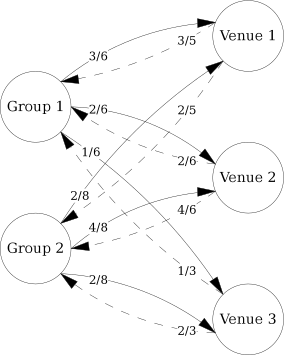
\includegraphics[width=5.2cm]{fig/bhrscore-w3}}
   \caption{Markov chain for an example with 2 research groups and 3 publication venues.}
   \label{fig:ex1-MC}
\end{figure}

From Figure \ref{fig:ex1-MC}, Group 1 published $3$ papers in venue $\mbox{v}_1$, $2$ papers in venue $\mbox{v}_2$, and $1$ paper in venue $\mbox{v}_3$. The number of publications of Group 1 is $6$. Venue $\mbox{v}_1$ receives $3$ papers of Group 1, and 2 papers of Group 2. The fractions of publications from groups to venues and from venues to groups are the edge weights.


%TODO
%... since publication venues are aggregations of papers and research groups are aggregations of authors.
%
%While Ribas has provided suggestions on how to instantiate the reputation graph to solve three common academic search tasks, we choose to...
%

%TODO cite ribas thesis
Ribas et al. also suggested different possible configurations for the reputation graph. In fact, the sources and collaterals can be any of the three types of entities we consider i.e., publication venues, authors, and research groups. The targets, however, must always be entities of type venues. That is, we should always use the reputation of venues as the key feature for ranking venues, research groups, and individual authors. 

In the next section, we present the initial approaches we adopted to rank academic entities on a per subarea basis and discuss our motivations to modify the standard P-score metric.


%%%%%%%%%%%%%%%%%%%%%
\section{The Encroachment Problem}\label{sec:encroachment}
%%%%%%%%%%%%%%%%%%%%%

Initially, based on the concepts and usability of the standard P-score, we consider a simple hypotesis: to rank academic entities on a per subarea basis, it would be sufficient to use the right reputation sources within a subarea and compute the steady state probabilities of all academic entities. As a result, in theory, the entities with higher P-scores would be the most reputable entities within a subarea. For instance, using as reputation sources the most important venues in Information Retrieval, we would find the most reputable authors, graduate programs, and publication venues in the subarea of IR.

Likewise, the instantiation of P-score in these first experiments, based on one of the possible configurations suggest by \citeauthor{ribas2015random}, was as follows: given a pre-selected set of reference venues (or \textit{seeds}) in a given subarea, e.g. conferences and/or journals, the metric finds the $n$ researchers with the largest volume of publications in these reference venues (for instance, $n$ = 200) and uses them to assemble the Markov network model which also includes all venues in which they published. The steady state probabilities are interpreted as venue weights which distinguish high reputation venues from the others. Thus, these weights can be used to rank venues (by considering these weights as venue scores) and also to rank research groups or authors.

%TODO 
%P-score ranks groups according to Equation~(\ref{eq:pscore_group_author}). 

However, this approach proves to be inappropriate when considering subareas. The reason is that publication venues possibly cover multiple subareas and thus their reputation need to be split among its component subareas. One example of such venue is the ACM Conference on Information and Knowledge Management (CIKM). It is a high reputation venue that covers three subareas: Databases (DB), Information Retrieval (IR), and Knowledge Management (KM). If we are interested in the subarea of IR in particular, we need to find a way to discount or weigh down the contributions of CIKM papers that are not on IR. If we do not, we might end with large P-score contributions to a given subarea, such as IR, from papers that are really on another subarea, such as DB. This is what we call the \textit{encroachment problem}. 

We illustrate with an example. Elisa Bertino is a well known and respected researcher who has published over 800 papers. Her interests cover many areas with focus on the fields of Information Security and DB systems. She has papers on CIKM and other venues that also accept papers on IR. Because of that she appears on the list of authors that publish frequently on IR related venues. And, because of the large number of papers she publishes her P-score on IR is high, which leads to a high rank of her group at Purdue University on the subarea of IR.

Given CIKM does not distinguish in its proceedings which papers are on IR, on DB or on KM, determining whether a given CIKM paper is on IR, for instance, would require examining its text contents. However, P-score is a metric that does not rely on paper contents -- one of its inherent advantages given it is much simpler to compute than citation-based metrics. Thus, imposing the need to have access to the contents of papers is a constraint we purposely want to avoid. Therefore, we look for a different solution, described in the next section.


%%%%%%%%%%%%%%%%%%%%%
\section{Normalized P-score for Publication Venues}\label{sec:npscore}
%%%%%%%%%%%%%%%%%%%%%

As our primary goal is to perform analysis of academic entities on a per subarea basis, it is crucial to investigate how we could identify suitable publication venues to characterize subareas. 

As originally proposed, P-score venue weights do not allow distinguishing venues in a given subarea, even if we choose as seeds venues that are central to that subarea (i.e. venues which are assuredly focused on that subarea). This occurs because P-score is a metric strongly correlated to the volume of publications. In other words, venues with high popularity that are related to the seeds -- i.e. have papers written by the authors used as seeds (or references) in the network -- are put in the top positions by the raw P-score.
%TODO seeds as authors or venues may become confusing to the reader

To avoid this problem, we normalize the venue's P-score by the number of publications in the venue's history. The key idea is to obtain an average of the overall reputation of the venue on a per paper basis. This approach penalizes venues with a large volume of publications but with low P-scores (low reputation according to the seeds) and boosts smaller publication venues with good reputation in a given subarea. Thus, the \textit{normalized P-score} for venue $v$ is defined as: 

\begin{equation}\label{eq:pscore_venue}
    \textit{norm-P-score($v$)} = \frac{\textit{P-score($v$)}}{\textit{number\_of\_publications}(v)}
\end{equation}

Equation (\ref{eq:pscore_venue}) is the starting point for obtaining the ranking of groups on a per subarea basis as presented in the following sections. 


%%%%%%%%%%%%%%%%%%%%%
\section{Weighted P-score for Research Groups}\label{sec:wpscore}
%%%%%%%%%%%%%%%%%%%%%

%TODO State clearly what is legacy and what we propose 
%TODO We could rewrite equations... 

To help understanding the modifications of standard P-score we propose for ranking research groups by subareas, let us rewrite some equations of standard P-score in a clearer and more concise way than using the whole conceptual framework of reputation flows, focusing on the group ranking itself.

Evaluating a research group, such as the researchers in Information Retrieval of a given CS graduate program, requires weighting the contributions of its members who are responsible for the reputation of the group. As \citeauthor{ribas2015random}, we say that the group's reputation is the sum of the reputation of the venues the members of the group published in, taken on a per author basis. Moreover, a research publication is usually a combination of efforts by multiple researchers. In consequence, we should normalize the paper's P-score by the number of authors. 
%Let $f(x)$ be any function that measures the reputation of an academic entity $x$. 
Thus:

\begin{equation}\label{eq:pscore_group}
    \textit{P-score($g$)} = \sum_{p \in \delta(g)} \frac{\textit{P-score(venue(p))}}{\textit{number\_of\_authors}(p)}
\end{equation}
where $\delta(g)$ are the publications of group $g$ and \textit{venue(p)} is the venue at which paper $p$ was published.
%
In other words, the reputation of a research group is based on the papers it published. Each paper has a reputation itself, which is given by the venue where the paper was published. 

The members of a research group are professors, postdoctoral fellows, doctoral students, among others. Normally, professors are responsible for the research groups at which postdoctoral fellows and doctoral students work. At some point, the group publishes a paper and the responsible professor is typically involved. This allows us to use professors as the anchors for transferring reputation to the research group. Notice that the indication of the author's affiliation is key to estimate reputation for groups. Hence, Equation~(\ref{eq:pscore_group}) may be rewritten as:

\begin{equation}\label{eq:pscore_group_author}
    \textit{P-score($g$)} = \sum_{a \in \varphi(g)} \sum_{p \in \delta(a)}  \frac{\textit{P-score(venue(p))}}{\textit{number\_of\_ authors}(p)}
    % \frac{\textit{P-score($v\ |\ v\ \in$ venue(p))}}{\textit{number\_of\_ authors}(p)}
\end{equation}
where $\varphi(g)$ are the researchers associated with group $g$ and $\delta(a)$ are the publications of author $a$. 

The equation~\ref{eq:pscore_group_author} is an alternative way of showing how the standard P-score metric ranks research groups, as stated by Equation~\ref{eq:pscore}, in Section~\ref{sec:flows}. Recap that standard P-score does not provide good ranking of research groups on a per subarea basis, due to the encroachment problem described in Section~\ref{sec:encroachment}. 

The solution we propose is to examine the main subareas of interest of each researcher and produce weights for the pairs $[researcher, subarea]$. We do so by examining the publications of the researchers on venues that are specific to a single subarea such as SIGIR and SIGMOD, for instance. Our rational is that a researcher that publishes eight SIGIR papers and two SIGMOD papers is focused on IR $80\%$ of the time and on DB 20\% of the time. 
%
In other words, this researcher interest factor on IR is 0.8 and on DB is 0.2. We then use this \textit{subarea interest factor} (hereinafter presented as $\gamma_{f}$) to weigh the papers of this author in venues that cover multiple subareas, such as CIKM. That is, instead of solving a classification problem (determine the subarea of each CIKM paper) which would require access to paper contents, we propose a ranking solution that ranks CIKM papers on each of its subareas based on their authors interest factors. Our ranking solution simplifies the implementation and leads to good results, as discussed in Chapter~\ref{sec:results}.

Let $S_{f}$ be a set of venues closely associated with subarea $f$ and $\delta(a)$ be the set of publications of author $a$, as before. Then:
\begin{equation}\label{eq:author_factor}
    \gamma{f}(a) = \frac{1}{\delta(a)} \sum_{p \in \delta(a)}
    \begin{cases}
         1 & \mbox{if $p \in S_{f}$}\\ 
         0 & \mbox{otherwise} 
    \end{cases}
\end{equation}
where $\gamma_{f}(a)$ is the weight of author in subarea $f$, i.e., a measure of how much the author belongs to that subarea.
% and $\delta(a)$ is the set of publications of author $a$. The results are bound within the interval $[0,1]$, where $1$ means that the author only published in the venues of the subarea (represented by $S_{f}$), and $0$ that she has none publication in the subarea.

Factor $\gamma$ quantifies the relation of authors to a given subarea, but does not take into account the history of publications by a given author. 
If an author changes their field of study, we should factor in that the author's relation to the subarea of interest has weakened. We do so by introducing a publication age penalty, as follows:
\begin{equation}\label{eq:author_factor_year}
    \gamma_{f}(a) = \frac{1}{\delta(a)} \sum_{p \in \delta(a)}
    \begin{cases}
      %\varepsilon - \varrho(p) + 1 & \mbox{if $p \in S_{area}$}  \\ 
    %   \frac{1}{\log_2 {(\varepsilon - \varrho(p) + 2)}} & \mbox{if $p \in S_{f}$} \\
      \frac{1}{\log_2 {(y(0) - y(p) + 2)}} & \mbox{if $p \in S_{f}$} \\
      0 & \mbox{otherwise} 
    \end{cases} \\ %y(p) \leq y(0) \\
\end{equation}
where $y(p)$ is the year in which the paper $p$ was published and $y(0)$ is the current year, or the year of the most recent paper in the collection. 

Using the subarea interest factor we can rewrite Equation~(\ref{eq:pscore_group_author}) and present the \textit{weighted P-score} of a group $\textit{g}$ in subarea $\textit{f}$ as:

\begin{equation}\label{eq:group_pscore_author_factor}
	\textit{weighted-P-score($g$)}_f = \sum_{a \in \varphi(g)} \gamma_f(a) \times \sum_{p \in \delta(a)} \frac{\textit{P-score(venue(p))}}{\textit{number\_of\_authors}(p)}
\end{equation}
~

\subsection*{Comparing Research on Different Subareas}

Most analyses of this kind consist of analyzing the raw number of publications in each subarea. Likewise, they tend to select few venues that represent the area and then only consider them for the purpose of counting. In here, besides number of publications, we also consider the reputation of each venue, according to P-score. As shown in Section \ref{sec:pscore}, P-score provides encouraging results in ranking academic entities. We aim to show that this metric, when applied to CS graduate programs, allows us to gain valuable insights about the divergences in current publication behavior between different countries.

One final caveat. When we compute P-scores on a per subarea basis, we run a stochastic computation for each subarea. A direct side effect is that P-scores of each subarea, which represent steady state probabilities in a Markov network, are scaled up to sum up to $1$. For comparisons among subareas, this is a problem. In particular, smaller venues might receive disproportionately high relative P-scores due to stochastic scaling in a given subarea. 

Thus, to allow proper comparisons across subareas, we use an artifact we borrow from the computation of Pagerank \citep{page98pagerank}. Inside each subarea, we consider that a fraction of the time, $85\%$ for instance, transitions occur to nodes inside the Markov network for that subarea. The other fraction of the time, $15\%$ for instance, transitions occur to nodes in one of the other subareas. The end result is that steady state probabilities of nodes in all subareas must now sum up to 1, which makes them directly comparable. 

%%%%%%%%%%%%%%%%%%%%%
%TODO \section{An Example}
%%%%%%%%%%%%%%%%%%%%%

%%%%%%%%%%%%%%%%%%%%%
%\section{Summary}
%%%%%%%%%%%%%%%%%%%%%

%%%%%%%%%%%%%%%%%%%%%%%%%%%%%%%%%%%%%%%%%%
\chapter{Experimental Setup}\label{sec:setup}
%%%%%%%%%%%%%%%%%%%%%%%%%%%%%%%%%%%%%%%%%%

In this section, we describe the setup supporting our experiments and the key assumptions we have considered on assessing reputation in academia. Specifically, we provide details of the academic dataset we used in this work, the definition of CS subareas, the methods we adopted, and previous results used as starting points to our present analysis.

%%%%%%%%%%%%%%%%%%%%%
\section{Dataset}
%%%%%%%%%%%%%%%%%%%%%
% [Characterize DBLP dataset and its enrichment (groups I and csrankings II)]

% # Papers = 2.931.849 | 4.551.362
% # Venues = 5.765
% # Authors = 1.595.771

We compiled a collection of academic publications records extracted from DBLP,\footnote{\url{http://dblp.uni-trier.de}} an online reference for bibliographic information on major CS publications. DBLP data has been used in related studies on CS research communities~\citep{wainer13, biryukov10, hoonlor13}. 
%
The database is publicly available in XML format and contains more than three million publication records from more than 1.5 million authors over the last 50 years, albeit the data before 1970 is rather irregular. Each publication record includes a title, list of authors, year of publication, and publication venue. Publication records do not include the contents of the papers neither information related to citation.

Our collection is actually an extension of the DBLP repository. While it contains all publication venues and authors from DBLP, we have enriched it adding information regarding research groups. To do so, we manually collected information about the top 126  CS graduate programs evaluated in the 2011 assessment conducted by the US National Research Council (NRC).\footnote{\url{http://www.nap.edu/rdp/}}
%
In particular, for each of these groups we retrieved the list of group members, which were then manually reconciled against the repository.

Despite our efforts, there were still imprecisions related to the affiliation of the authors. To address them, we combined our dataset with the one provided by the \textit{csranking} project,\footnote{\url{http://csrankings.org/}} which ranks CS departments based purely on their publications.They do so by collaboratively collecting information on authors, such as their homepage and affiliation. Therefore, we used that information to enhance our repository. Salient statistics on our dataset are shown in Table~\ref{tab:stats}.

\begin{table}[htbp]
\centering
\caption{Salient statistics of the dataset used in our evaluation.}
\label{tab:stats}
\begin{tabular}{l|r}
\toprule
Attribute & Value \\ \hline
Number of Papers         & $2{,}931{,}849$                 \\
Number of Authors        & $1{,}595{,}771$                 \\
Number of Venues         & $5{,}765$                     \\
Number of US Depts		 & $126$                       \\
Avg. number of professors per US Dept	&	$42.4$				              \\ % 5347 / 126 
Number of BR Depts    							            & $25$                        \\
Avg. number of professors per BR Dept	&	$47.8$				              \\ % 1196 / 25
\bottomrule
\end{tabular}
\end{table}


%%%%%%%%%%%%%%%%%%%%%
\section{Computer Science Subareas}
%%%%%%%%%%%%%%%%%%%%%

There are different ways of defining subareas in CS, %it may depend on time and also 
depending on the institution responsible for the classification. Two notorious classification are given by ACM\footnote{\url{http://acm.org/sigs}} (through \textit{Special Interest Groups}) and IEEE\footnote{\url{http://computer.org/web/tandc/technical-committees}} (through \textit{Technical Committees}). 
%One thing that is important to 
Notice that most of them divide CS into subareas rather distinct. Further, some of these divisions reflect historical decisions that may be less relevant nowadays. For this reason, 
previous works have attempted to automatically identify such subareas~\citep{wainer13} or use other source of information~\citep{hoonlor13}.

% In this work, we adopt the classification of CS subareas provided by Microsoft Academic 
% Research.\footnote{\url{http://academic.research.microsoft.com}} This classification divides CS in 37 subareas, including relatively new subareas such as Knowledge Management and Natural Language Processing. The full list of subareas are presented in Table~\ref{tab:subareas}.

A more recent classification is presented by Microsoft Academic Research.\footnote{\url{http://academic.research.microsoft.com}} They divide CS in 37 subareas, including relatively new subareas. For the purpose of this work, we selected 20 subareas from the Microsoft Academic Search classification, as presented in Table~\ref{tab:subareas}.

\begin{table}[h]
%\scriptsize
%\footnotesize
%\normalsize
\small
\centering
\caption{Subareas of Computer Science selected from Microsoft classification.}
\label{tab:subareas}
\begin{tabular}{l|c|l}
\toprule
Subarea 					 & Abbreviation & Seed venues          \\ \hline
Algorithm                    & Alg          & SODA, Algorithmica   \\ \hline
Artificial intelligence      & AI           & IJCAI, AI            \\ \hline
Bioinformatics               & Bio          & BIBM, Bioinformatics \\ \hline
Computer graphics            & CG           & SIGGRAPH, TCVG       \\ \hline
Computer network             & CN           & INFOCOM, TON         \\ \hline
Computer security            & CS           & CCS, TISSEC          \\ \hline
Computer vision              & CV           & CVPR, IJCV           \\ \hline
Data mining                  & DM           & KDD, SIGKDD          \\ \hline
Database                     & DB           & SIGMOD, TODS         \\ \hline
Distributed computing        & DC           & ICDCS, TPDS          \\ \hline
Human-computer interaction   & HCI          & CHI, TOCHI           \\ \hline
Information Retrieval        & IR           & SIGIR, TOIS          \\ \hline
Machine learning             & ML           & ICML, JMLR           \\ \hline
Natural language processing  & NLP          & EMNLP, COLING        \\ \hline
Operating system             & OS           & SOSP, SIGOPS         \\ \hline
Parallel computing           & PC           & IPPS, TPDS           \\ \hline
Programming language         & PL           & PLDI, TOPLAS         \\ \hline
Speech Recognition           & SR           & INTERSPEECH, TCOM    \\ \hline
Theoretical computer science & TCS          & STOC, SIAMCOMP       \\ \hline
World Wide Web               & WWW          & WWW, WS              \\ 
\bottomrule
\end{tabular}
\end{table}

Along with the list, we present the abbreviation of each subarea, which we will be using from here on. We also show two venues we selected as notorious and is associated specifically with the subarea of interest, which are essential for identifying a group of researchers whose main research topics of interest,are likely to be in that subarea -- an essential information for the connect application of P-score to subareas. 
%
We avoided using all 37 subareas because we found some of them difficult to characterize. While our subset of 20 CS subareas is not perfect or exhaustive, it is detailed enough to allow gaining insights into the scene of research in CS in Brazil, which would not be possible to obtain otherwise. In Appendix~\ref{sec:cs-subareas}, we present other classifications of CS subareas, according to other reliable sources.

%TODO connect application, is that right? 


%%%%%%%%%%%%%%%%%%%%%
\section{Venues Ground-Truth}\label{sec:venue-ground-truth}
%%%%%%%%%%%%%%%%%%%%%

To evaluate the effectiveness of normalized P-scores from Equation (\ref{eq:pscore_venue})  on the task of finding venues in a subarea, we considered as ground-truth the opinion of experts. Specifically, we asked reputable CS researchers and their graduate students, working on subareas of IR, DB and Data Mining (DM) to asses the relevance to their subarea of venues included in a pre-selected list. This list consists of the venues at the top 50 positions in the P-score ranking, when we use as seeds two publication venues only: a journal and a conference closely associated with that subarea. For examples of seeds, see Table~\ref{tab:seeds}.

\begin{table}[htbp]
\centering
\caption{Seeds of publication venues for P-score used in this work.}
\label{tab:seeds}
\begin{tabular}{l|ccc}
\toprule
                                   & \multicolumn{3}{c}{Subareas}                                                            \\ \hline
\multicolumn{1}{c|}{Type of venue} & \multicolumn{1}{c|}{Database} & \multicolumn{1}{c|}{Data Mining} & Information Retrieval \\ \hline
\multicolumn{1}{l|}{Conference}    & \multicolumn{1}{c|}{SIGMOD}   & \multicolumn{1}{c|}{KDD}         & SIGIR                 \\ \hline
\multicolumn{1}{l|}{Journal}       & \multicolumn{1}{c|}{TODS}     & \multicolumn{1}{c|}{SIGKDD}      & TOIS                 \\
\bottomrule
\end{tabular}
\end{table}

We thus focused on the CS subareas of  DB, DM and IR. For each subarea, three experts have classified each of the 50 venues of the pre-selected list into one, two or three subareas chosen among the 37 subareas listed in Table~\ref{tab:subareas}. To reconciliate the multiple classifications, we used a majority criterion: if a publication venue $v$ was associated with a subarea $s$ at least twice, $s$ was considered one of the subareas of $v$. Hereafter, we will refer to the full lists of publication venues and their subareas as our \textit{venues ground-truth}.

% As a result, that allows us to perform a precision-recall analysis of different approaches in finding venues given a subarea, as show in Figure~\ref{fig:norm-pscore-curves}. For the evaluation, we have considered only the same 50 publication venues already classified by the experts. For this reason, all strategies reach the maximum recall (100\%) at the end of each curve. We used the H-index metric and the standard P-score as competitors for the normalized P-score. For the both metrics based on the P-score, we chosen the same initial seeds of reputation, as shown in the Table~\ref{tab:seeds}.

%TODO other filterings
% Venues: min-pub=100, live-in:2012

%TODO
%%%%%%%%%%%%%%%%%%%%%
%\section{Evaluation Methodology}
%%%%%%%%%%%%%%%%%%%%%
%\subsection*{Ranking Venues}\label{sec:eval-venues}
%Competitors: 
%
%H-index
%
%Standard P-score
%
%H-indices were obtained from Google Scholar.
%
%using the conference SIGIR and the journal TOIS as reputation references.
%
%\subsection*{Ranking Research Groups}\label{sec:eval-groups}

%%%%%%%%%%%%%%%%%%%%%
%\section{Summary}
%%%%%%%%%%%%%%%%%%%%%


%%%%%%%%%%%%%%%%%%%%%%%%%%%%%%%%%%%%%%%%%%
\chapter{Experimental Results}\label{sec:results}
%%%%%%%%%%%%%%%%%%%%%%%%%%%%%%%%%%%%%%%%%%

%TODO
In this chapter, we discuss the results of ranking publication venues and research groups in CS on the three subareas we selected: Information Retrieval, Databases, and Data Mining. In particular for ranking of groups, our results are restricted to the 126 US graduate programs considered by NRC in 2011.

In particular, in this chapter we aim to answer the research question Q1) \textit{How to quantify the reputation of publication venues and research groups on a per subarea basis?}. In Sections \ref{sec:results-us} and \ref{sec:results-br} we intend to answer the research question Q2) \textit{How does the reputation of Brazilian and US graduate programs in CS vary per subarea?}. Lastly, in Section \ref{sec:comparison}, we discuss about question Q3) \textit{Are there differences between the current research directions in CS of the top Brazilian and US graduate programs?}

%%%%%%%%%%%%%%%%%%%%%
\section{Ranking Venues}\label{sec:results-venues}
%%%%%%%%%%%%%%%%%%%%%

Using the normalized P-score (norm-P-score) presented in Section \ref{sec:npscore}, we were able to better discriminate publication venues of a given CS subarea from venues of other subareas. Figure~\ref{fig:norm-pscore-curves-ir} presents the precision-recall curve obtained by norm-P-score in the task of ranking publication venues in Information Retrieval, in light of the results produced using two other methods, namely H-index and standard P-score. %, as described in Section \ref{sec:eval-venues}. 
To produce the precision-recall curves, we use as ground-truth a classification of venues manually set by experts in each subarea, as explained in Section ~\ref{sec:venue-ground-truth}. 
We reproduced the same experimental methodology for ranking venues in the subareas of Databases and Data Mining. The precision-recall curves are shown in Figure \ref{fig:norm-pscore-curves-db-dm}.

\begin{figure}[htbp]
	\centering
    \label{fig:norm-pscore-curves-ir}
    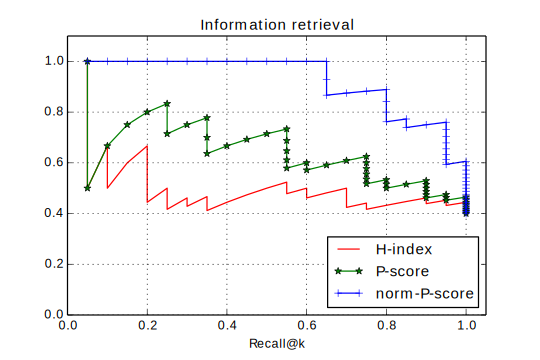
\includegraphics[width=0.8\linewidth]{fig/ir-prec-recall.eps}
    \caption{Precision-Recall curves of H-index, P-score and normalized P-score for the subarea of Information Retrieval.}
\end{figure}

\begin{figure}[htbp]
	\centering
    \label{fig:norm-pscore-curves-db-dm}
    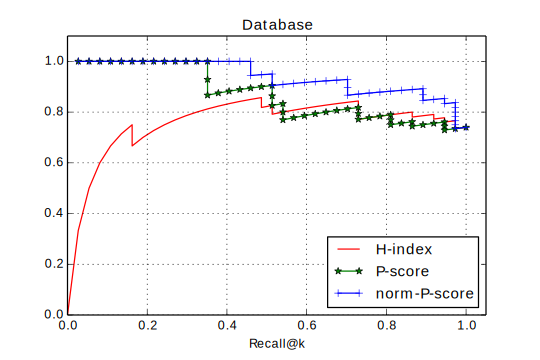
\includegraphics[width=0.8\linewidth]{fig/db-prec-recall.eps}
    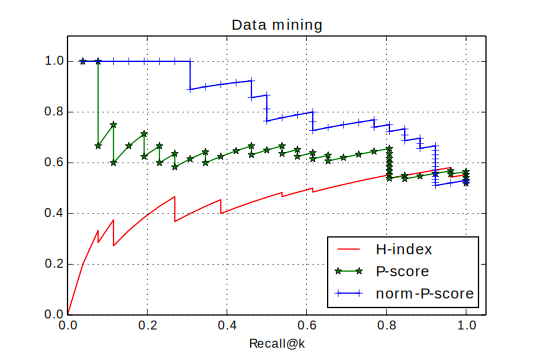
\includegraphics[width=0.8\linewidth]{fig/dm-prec-recall.eps}
    \caption{Precision-Recall curves of H-index, P-score and normalized P-score for the subareas of Database and Data Mining.}
\end{figure}

%TODO put the rankings of venues for the other subareas? Appendix?

As it is clear from Figures \ref{fig:norm-pscore-curves-ir} and \ref{fig:norm-pscore-curves-db-dm}, normalized P-scores allow identifying the correct venues consistently better than H-indices and standard P-scores. Furthermore, for all the three subareas, the normalized P-scores yield maximum precision ($100\%$) for the initial $30\%$ of recall. This 
means that the first 15 venues in the normalized P-score ranking are strongly related to IR, according to the assessments of specialists.

To further illustrate, Table~\ref{tab:ir-venues} shows the top 20 publication venues for the subarea of IR, produced by P-scores and normalized P-scores when we consider SIGIR and TOIS as seed venues. 
%
On the one hand, the standard P-score metric places venues such as the International World Wide Web Conferences (WWW) and the International Conference on Multimedia (MM), among the top 10 positions. These two conferences cover topics of the subarea of IR, but indeed have a larger scope than IR only. 
%
On the other hand, such conferences do not appear in the normalized P-score ranking, even among the top 20 positions on the ranking. Besides, in the normalized P-score ranking, venues mainly focused in IR venues such as the International Conference on the Theory of Information Retrieval (ICTIR) and Transactions on Information Systems (TOIS) appear among the top 10 publication venues. In particular, ICTIR appears at the top. This power of discrimination of the normalized P-score is important to allow selecting venues that better represent the subarea of IR.

\begin{table}[htbp]
\centering
\caption{Top 20 venues in Information Retrieval, using P-score and normalized P-score. The suffixes (c) and (j) are used to differentiate conferences and journals with the same name.}
\label{tab:ir-venues}
%\resizebox{\columnwidth}{!}{%
\begin{tabular}{rcc}
	\toprule
	%\multicolumn{2}{c|}{Database} & \multicolumn{2}{c|}{Data Mining} & \multicolumn{2}{c}{Information Retrieval} \\ \hline
	\#	& P-score 	& Norm-P-score \\ \hline
	1	& SIGIR (c)	& ICTIR \\ 
	2	& CIKM	        & SIGIR (c) \\ 
	3	& TREC	        & ADCS              \\ 
	4	& ECIR	& IR \\ 
	5	& CLEF	& ECIR \\ 
	6	& WWW	& TREC \\ 
	7	& JASIS	& SIGIR (j) \\ 
	8	& IPM	& IIIX \\ 
	9	& SIGIR	(j) & TOIS \\ 
	10	& MM	& WSDM \\ 
	11	& JCDL	& INEX \\ 
	12	& TOIS	& SPIRE \\ 
	13	& IR	& AIRS \\ 
	14	& WSDM	& CIKM \\ 
	15	& NTCIR	& TWEB \\ 
	16	& KDD	& RIAO \\ 
	17	& TKDE	& CLEF \\ 
	18	& ACL	& NTCIR \\ 
	19	& ICDM	& LA-WEB \\ 
	20	& SPIRE	& JCDL \\ 	
	\bottomrule
\end{tabular}
\end{table}

It is noteworthy to mention that the normalized P-score ranking of venues should not be interpreted as an impact or productivity ranking. We only use this output to define the most representative venues of a subarea, in a semi-automatic fashion.

Afterward, using this ranking of publication venues as starting point, we can subsequently improve rankings of graduate programs in CS by considering a per subarea basis. Our results in ranking graduate programs are discussed in the next Section.

%%%%%%%%%%%%%%%%%%%%%
\section{Ranking US Graduate Programs by Subarea}\label{sec:results-us}
%%%%%%%%%%%%%%%%%%%%%

For this section, we are interested in the distribution of publications in the CS subareas of graduate programs across US. More specifically, we want to understand which subareas receive more attention by the top graduate programs in US. 

%P-score provides good rankings of venues~\citep{ribas2015random}, however, rankings of groups using standard P-score are disrupted by the encroachment discussed in Section~\ref{sec:encroachment}. In a broad area as CS, one should consider each subarea separately rather than evaluating the whole area, since they are not the same. Therefore, we propose to rank US graduate programs considering subareas. 
As in Section \ref{sec:results-venues}, we consider the same three CS subareas: IR, DB, and DM.

%%%%%%%%%%
\subsection*{Information Retrieval, Databases, and Data Mining}
%%%%%%%%%%
%% IR 
Table~\ref{tab:top10-ir-pscore} presents a ranking of groups using standard P-scores for IR. The values presented are normalized to $1$ as follows:
\begin{equation}\label{eq:norm-values}
    \overline{P}(g)_{f} = \frac{P(g)_{f}}{max(P(g)_{f})}
\end{equation}
where $\overline{P}(g)_{f}$ is the normalized score of group $g$ in $f$, $P(g)_{f}$ is the score and $max(P(g)_{f})$ is the highest score. We apply Equation~\ref{eq:norm-values} to either standard and weighted P-scores.

\begin{table}[htbp]
\centering
\caption{Ranking of the top 10 US Universities on Information Retrieval, using standard P-scores.}
\label{tab:top10-ir-pscore}
\begin{tabular}{rlr}
	\toprule
	\# & University                                 & \multicolumn{1}{c}{P-score} \\
	\midrule
	1  & Carnegie Mellon University                 & $1$            \\
	2  & University of Massachusetts Amherst        & $0.8082$ \\
	3  & University of Illinois at Urbana-Champaign & $0.6735$ \\
	4  & University of Southern California          & $0.4541$ \\
	5  & Georgia Institute of Technology            & $0.4341$ \\
	6  & Stanford University                        & $0.3493$ \\
	7  & University of Illinois at Chicago          & $0.3409$ \\
	8  & Cornell University                         & $0.3344$ \\
	9  & University of California-Berkeley          & $0.3337$ \\
	10 & Purdue University                          & $0.3120$ \\
	\bottomrule
\end{tabular}
\end{table}

The University of Massachusetts Amherst has the premier research group IR in the US and thus, the fact that it was not in first place in the rank was surprising to us. This led to an in-depth analysis of the ranking and the consequent understanding of the encroachment problem, as discussed in Section~\ref{sec:encroachment}. 
%
Tables~\ref{tab:top10-ir} presents the top 10 universities on IR using our proposed approach of the weighted P-score, according to Equation~(\ref{eq:group_pscore_author_factor}), instead. We observe that the University of Southern California, the Georgia Institute of Technology, Stanford University and the University of California at Berkley are no longer among the top 10 IR groups. This seems appropriate given these universities are not active on research in IR.

\begin{table}[htbp]
\centering
\caption{Ranking of the top 10 US Universities on Information Retrieval, using the weighted P-score (Equation~\ref{eq:group_pscore_author_factor}).}
\label{tab:top10-ir}
\begin{tabular}{rlr}
	\toprule
	\# & University                                 & \multicolumn{1}{c}{weighted-P-score} \\
	\midrule
	1  & University of Massachusetts Amherst        & $1$                         \\
	2  & University of Illinois at Urbana-Champaign & $0.4830$                    \\
	3  & Carnegie Mellon University                 & $0.4625$                    \\
	4  & University of Delaware                     & $0.2452$                    \\
	5  & Purdue University                          & $0.2276$                    \\
	6  & Northeastern University                    & $0.1633$                    \\
	7  & Lehigh University                          & $0.0964$                    \\
	8  & Cornell University                         & $0.0552$                    \\
	9  & University of Iowa                         & $0.0494$                    \\
	10 & University of Illinois at Chicago          & $0.0477$                    \\
	\bottomrule
\end{tabular}
\end{table}

To better understand the results in Table~\ref{tab:top10-ir}, we produced a list of the top 20 researchers on IR. Table~\ref{tab:top-authors} shows their affiliation. As we observe, our top 10 IR groups are those whose researchers are also among the top 20 authors on IR in the US. In particular, the top 3 groups have each one 2 or more researchers among the top 20. 
%
We also manually examined our ranking of authors to observe that the top authors shown in Table~\ref{tab:top-authors} had more publications in venues strongly related to the subarea. Hence, the ranking of groups can be justified by the ranking of authors. 

\begin{table}[htbp]
\centering
\caption{Ranking of the top 20 US authors' universities on Information Retrieval, using Equation~(\ref{eq:group_pscore_author_factor}).}
\label{tab:top-authors}
\begin{tabular}{rl}
	\toprule
	\# & Authors' universities \\
	\midrule
	1  & University of Massachusetts Amherst \#1        \\
	2  & University of Massachusetts Amherst \#2        \\
	3  & Carnegie Mellon University \#1                 \\
	4  & University of Illinois at Urbana-Champaign \#1 \\
	5  & Purdue University                            \\
	6  & University of Delaware                       \\
	7  & Northeastern University                      \\
	8  & University of Illinois at Urbana-Champaign \#2 \\
	9  & Lehigh University                            \\
	10 & Carnegie Mellon University \#2                 \\
	11 & University of Iowa                           \\
	12 & University of Illinois at Chicago            \\
	13 & Georgia Institute of Technology              \\
	14 & University of Virginia                       \\
	15 & Carnegie Mellon University \#3                 \\
	16 & Texas A\&M University                        \\
	17 & Cornell University                           \\
	18 & University of Michigan                       \\
	19 & University of Massachusetts Amherst \#3        \\
	20 & New York University                          \\
\bottomrule
\end{tabular}
\end{table}

We repeated this process to the subareas of DB and DM. Tables~\ref{tab:top10-db} and~\ref{tab:top10-dm} present the top 10 universities on DB and DM, when we use the weighted P-scores produced by Equation~(\ref{eq:group_pscore_author_factor}).

\begin{table}[htbp]
\centering
\caption{Ranking of the top 10 US Universities on Databases, using the weighted P-score (Equation~(\ref{eq:group_pscore_author_factor})).}
\label{tab:top10-db}
\begin{tabular}{rlr}
	\toprule
	\# & University                                 & \multicolumn{1}{c}{weighted-P-score} \\
	\midrule
	1	& University of Wisconsin-Madison				& $1$	    \\
	2	& Stanford University							& $0.6570$	\\
	3	& University of Illinois at Urbana-Champaign	& $0.5687$	\\
	4	& Massachusetts Institute of Technology			& $0.4975$	\\
	5	& Duke University								& $0.4616$	\\
	6	& University of Massachusetts Amherst			& $0.4243$	\\
	7	& University of Michigan						& $0.4195$	\\
	8	& University of California-Irvine				& $0.4120$	\\
	9	& University of Maryland-College Park			& $0.4101$	\\
	10	& University of California-Santa Cruz			& $0.3982$	\\
	\bottomrule
\end{tabular}
\end{table}

\begin{table}[htbp]
\centering
\caption{Ranking of the top 10 US Universities Data Mining, using the weighted P-score (Equation~(\ref{eq:group_pscore_author_factor})).}
\label{tab:top10-dm}
\begin{tabular}{rlr}
	\toprule
	\# & University                                 & \multicolumn{1}{c}{weighted-P-score} \\
	\midrule
	1	& University of Illinois at Chicago				& $1$	    \\
	2	& Carnegie Mellon University					& $0.6857$	\\
	3	& University of Illinois at Urbana-Champaign	& $0.6344$	\\
	4	& University of Minnesota						& $0.5350$	\\
	5	& Arizona State University						& $0.4276$	\\
	6	& University of California-Riverside			& $0.4212$	\\
	7	& Georgia Institute of Technology				& $0.3955$	\\
	8	& University of Michigan						& $0.3275$	\\
	9	& Rensselaer Polytechnic Institute				& $0.2761$	\\
	10	& University of California-Davis				& $0.2593$	\\
	\bottomrule
\end{tabular}
\end{table}

Our analysis on a per subarea basis uncovers venues and research groups that are not always thought of as high excellence. But, once one considers their track records on a specific subarea, it is clear that they are quite productive. That is, analyzing research groups on a per subarea basis yields insights that are hidden when we apply global metrics of productivity to a broad area as CS.

%%%%%%%%%%
\subsection*{US Research Overview}
%%%%%%%%%%

For the results presented here, we used the weighted-P-score (Equation~\ref{eq:group_pscore_author_factor}) to rank graduate programs in the 20 subareas selected. To do so, we first got the P-score for each subarea, where we used as seeds the venues in Table~\ref{tab:subareas}. After that, normalized P-scores allowed us to select the top venues that more adequately represent each subarea. Following, we used them to compute the weighted-P-score for each graduate program in each subarea. Finally, we selected the top 20 graduate programs in US, for each subarea. Figure \ref{fig:us-research} presents the results we obtained.

Figure~\ref{fig:us-research} presents our experiments considering only CS graduate programs in the US. It shows the accumulated weighted-P-score for the top 20 CS graduate programs in each of the 20 subareas. We observe that Computer Vision is the subarea with highest accumulated weight-P-score, followed by Database, Theoretical Computer Science, and Machine Learning.

\begin{figure}[tb] %htbp
    \centering
    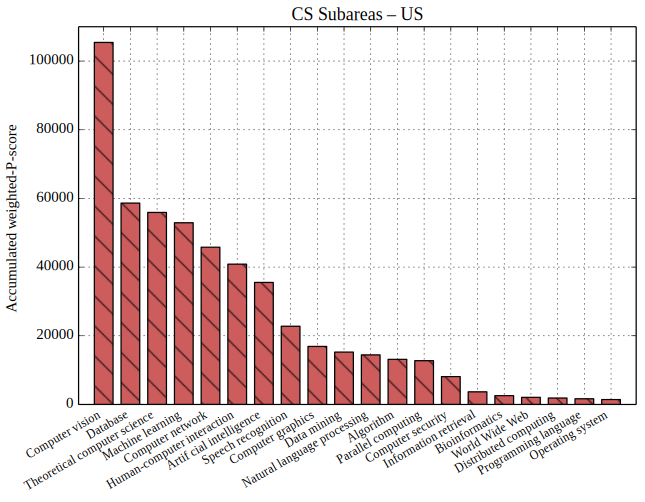
\includegraphics[width=0.9\linewidth]{fig/chart_usa_scaled.eps}
    \caption{Distribution of cumulative P-scores for the top 20 US graduate programs on a per subarea basis.}
    \label{fig:us-research}
\end{figure}

Computer Vision atracts a lot of attention and interest nowadays because it is present in some of the most cutting-edge technologies, such as autonomous vehicles which demand a massive amount of computer vision processing. On the other hand, Theoretical CS may appear a bit surprising. It is an area where publishing is slightly more difficult, especially because it often demands time, e.g. to prove theorems, and faculty usually advise fewer students and are thus likely to produce fewer papers~\citep{wainer13}. Despite this, our experiments showed TCS in third place. When inspecting the number of publications, we noticed that they have fewer than others, indeed. However, P-scores for venues in TCS were rather significant, indicating that the subarea has various venues of high reputation.

Another surprising subarea observed from Figure~\ref{fig:us-research} is Machine Learning. While it is a remarkable growing field of study, we observed that P-scores of ML venues were not well distributed. One problem that we noticed is that ML is extremely multidisciplinary. This becomes a problem because it is harder to find pure venues dedicated exclusively to Machine Learning. Many subareas include Machine Learning related research, a good example is Computer Vision.

Database and Computer Network are also well positioned in our experiment. They are more traditional fields of study (TCS as well) and have a considerable amount of work developed in the past. 

%%%%%%%%%%%%%%%%%%%%%
\section{Ranking BR Graduate Programs by Subarea}\label{sec:results-br}
%%%%%%%%%%%%%%%%%%%%%

We apply the same methodology of Section~\ref{sec:results-us} for assessing the reputation of CS graduate programs in Brazil. Figure~\ref{fig:br-research} presents our findings. It shows the accumulated weighted-P-score for the top 20 CS graduate programs in each of the 20 subareas. According to our results, Parallel Computing is the subarea with highest accumulated weight-P-score (considerably higher than the others), followed by Information Retrieval and Computer Graphics.

\begin{figure}[tb]
    \centering    
    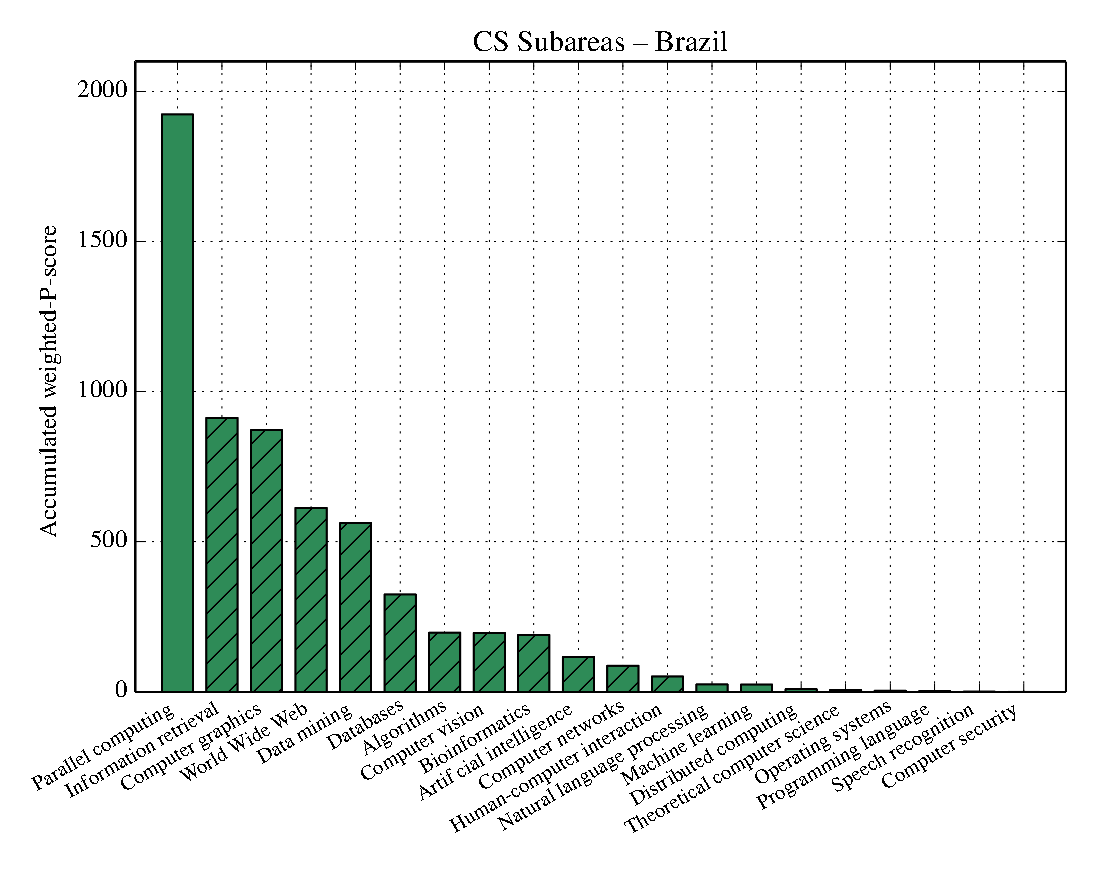
\includegraphics[width=0.9\linewidth]{fig/chart_br_scaled_sorted.eps}
    \caption{Distribution of cumulative P-scores for the top 20 BR graduate programs per subarea.}
    \label{fig:br-research}
\end{figure}

We also observe that P-scores for Brazil are almost two orders of magnitude smaller than those in the US. Thus, while volume of publications in Brazil is relatively high, see \citep{laender2008}, their impact in terms of exposure in high reputation venues is rather modest. 

Computer Science production in Brazil is considerably uneven. Many subareas have extremely low scores, in some of them, the score is almost inexistent. Thus, while there are researchers in Brazil working on all subareas, papers published in reputable venues, in various subareas are in rather small numbers. In constrast, we noted that in some CS subareas there are Brazilian graduate programs as reputable as the top US research groups. For instance, the Figure \ref{fig:ranking-ir} shows the top 20 graduate programs in Information Retrieval, according to the weighted-p-score. We observe two Brazilian research groups among these programs. This is noteworthy, given this kind of finding would not be possible without considering a per subarea basis.

\begin{figure}[htbp]
    %\centering
 	\includegraphics[width=\linewidth]{fig/ir_groups.eps}
    \caption{Top 20 Graduate Programs in Information Retrieval according to weighted-P-score, considering US and BR research groups, using logarithmic-scale.}
    \label{fig:ranking-ir}
\end{figure}

%%%%%%%%%%%%%%%%%%%%%
\section{Comparing BR and US Research in CS}\label{sec:comparison}
%%%%%%%%%%%%%%%%%%%%%

In Figure~\ref{fig:br-research-us-order} we reorder the results presented in Figure~\ref{fig:br-research} according to the subarea order in the US graduate programs in Figure~\ref{fig:us-research}, with the purpose of comparing the CS research scenario in the Brazil and in US.

\begin{figure}[tb]
    \centering
    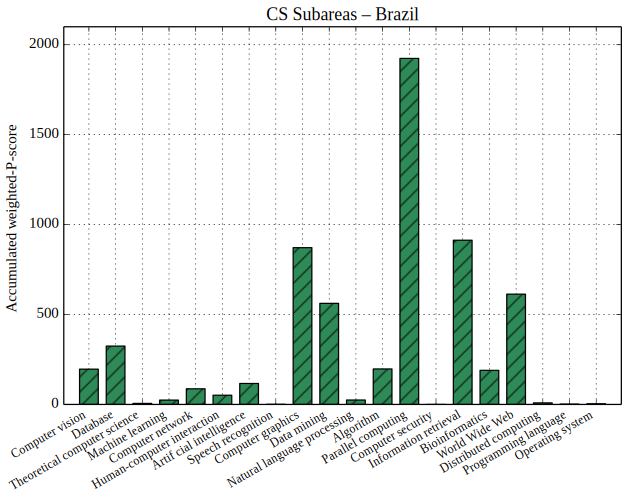
\includegraphics[width=0.9\linewidth]{fig/chart_br_scaled.eps}
    \caption{Distribution of cumulative P-scores for the top 20 BR graduate programs per subarea, in the same subarea order of Figure \ref{fig:us-research}.}
    \label{fig:br-research-us-order}
\end{figure}

In Brazil, Parallel Computing and Information Retrieval are the subareas with the highest scores, while in the US the top two subareas of greatest interest are Computer Vision and Database. 
%
We also observe that the top five subareas of greatest interest to Brazilian researchers are very distinct from those of greatest interest to US researchers. This suggests that academic research in Brazil is not shifting its focus of attention as fast as it happens in the US.

%%%%%%%%%%%%%%%%%%%%%
%\section{Summary}
%%%%%%%%%%%%%%%%%%%%%


%%%%%%%%%%%%%%%%%%%%%%%%%%%%%%%%%%%%%%%%%%
\chapter{Conclusions and Future Work}\label{sec:conclusions}
%%%%%%%%%%%%%%%%%%%%%%%%%%%%%%%%%%%%%%%%%%

In this dissertation, our first research question was: \textit{``How to quantify the reputation of publication venues and research groups on a per subarea basis?''} We presented experiments suggesting that metrics that only capture broad features of a subarea such as the volume of publications, citations or the general reputation (standard P-score included) are not sufficient to produce reasonable rankings in a per subarea basis. In particular, we demonstrated that solving the venues encroachment problem allows us to improve the ranking of research groups in a given subarea. We showed a simple but effective strategy to increase or decrease the contribution of an author to the overall reputation of her research group in a given subarea, based on the author's relation to that subarea. 

Our second research question was: \textit{``How does the reputation of Brazilian and US graduate programs in CS vary per subarea?''} We showed that the identification of the most reputable publication venues and graduate programs in Computer Science depends on the subarea considered to the task. Specifically, both the most suitable venues as the rankings of Brazilian and US departments vary on a per subarea basis, considering for instance the subareas of Information Retrieval, Databases and Data Mining. Besides, we described how to modify the P-score metric to find the core venues of a subarea in a semi-automatic fashion and, subsequently, how to rank research groups using this information, obtaining the top research groups of a given subarea.

Our third research question was: \textit{``Are there differences between the current research directions in CS of the top Brazilian and US graduate programs?''} We showed that, in terms of reputation, the current research of the top graduate programs in Brazil and US differ considerably. It is known that the volume of US scientific publications in CS is significant superior to the volume of Brazilian CS research. However, this work shows that the CS subareas in which each country has major scientific impact are basically disjoint. 
Moreover, the large distance between the reputation scores of Brazil and US programs emphasizes the focus of US researchers on publishing in the most reputable conferences and journals within their subareas. 

% In this paper, our first research question was: \textit{``How does the reputation of Brazilian graduate programs in CS vary per subarea?''} We showed that the definition of the most reputable Brazilian graduate programs in CS depends on the subarea we take into account. For instance, in Information Retrieval, there is a significant distance between the top 3 (?) programs and the others. Similar behaviour could be observed in the subareas of Databases and Computer Networks. Moreover, we showed that Brazilian graduate programs are concentrated in subareas such as  Computer Graphics, Information Retrieval and Parallel Computing. This kind of information provides insights to government funding agencies, university officials, department chairs on how to allocate research fundings. 

%TODO Rephrase / Introduction of conclusions?
%Our intent is to show that reputation flows can be used to gain insight into the productivity of individual researchers and of research groups, not that a ranking based on a single metric should be taken at face value. Instead, the decision on how to classify or rank individual researchers and research groups can only be made by committees composed of human specialists. However, even under this light, committees of specialists need data and metrics that can be used to support their decisions.
%
%Additionally, the framework of reputation flows provides a complementary view on the reputation of academic entities which allows implementation of new features, such as notification alerts on new venues with rising reputation, as discussed in Ribas et al. [2017].
%%

%%%%%%%%%%%%%%%%%%%%%
%\section{Summary of Contributions}
%%%%%%%%%%%%%%%%%%%%%

%%%%%%%%%%%%%%%%%%%%%
%\section{Summary of Conclusions}
%%%%%%%%%%%%%%%%%%%%%

%%%%%%%%%%%%%%%%%%%%%
%\section{Directions for Future Research}
%%%%%%%%%%%%%%%%%%%%%

For future work, we want to include academic data of other regions of the world, such as European and Asian graduate programs, and, thereupon, characterize the distribution of the most reputable graduate programs in CS worldwide, on a per subarea basis. Also, we expect to compare only more recent publications in the CS subareas (e.g. the last 5 years of scientific research), where we intend to observe the current interest of the CS community. Further, we intend to perform a more detailed temporal analysis of the evolution of the CS subareas communities over the years, looking for the shape of CS changes over time. Another further study is to validate the reputation model in other broad areas than CS, such as Economics, whose differences in publication patterns on a per subarea basis seem to be greater than in Computer Science.

%TODO Vardi: providing the public with relevant information.

%%%%%%%%%%%%%%%%%%%%%%%%%%%%%%%%%%%%%%%%%%
\ppgccbibliography{masters}
%%%%%%%%%%%%%%%%%%%%%%%%%%%%%%%%%%%%%%%%%%

\begin{appendices}
\chapter{Clustering Computer Science}\label{sec:clustering}
%%%%%%%%%%%%%%%%%%%%%%%%%%%%%%%%%%%%%%%%%%

% Clustering
Initially, we explored some clustering methods in order to help us characterize research communities. To do that, we built a graph of coauthorships, using the data from the DBLP dataset. In this graph, each node is a distinct researcher and each edge represents a cowork of the authors -- an article written by the both authors. The higher the number of collaborations between the authors, the greater the weight of the edge connecting them. We use this weight as a measure of collaboration among the authors. This allows us to run clustering algorithms and analyze the resulting communities, as we now discuss.

\section{Markov Cluster Algorithm}

One of the main algorithms used in our initial studies, the Markov Cluster Algorithm (MCL) discussed in \citep{mcl} is a fast and scalable unsupervised cluster algorithm for graphs based on simulation of stochastic flow in graphs. It finds cluster structures in graphs by a mathematical bootstrapping procedure. The process deterministically computes (the probabilities of) random walks through the graph, and uses two operators transforming one set of probabilities into another. It does so using the language of stochastic matrices (also called Markov matrices) which capture the mathematical concept of random walks on a graph.
The MCL algorithm simulates random walks within a graph by an alternation of two operators called expansion and inflation. The expansion coincides with taking the power of a stochastic matrix using the normal matrix product (i.e. matrix squaring). Inflation corresponds with taking the Hadamard power of a matrix (taking powers entrywise), followed by a scaling step, such that the resulting matrix is stochastic again, i.e. the matrix elements (on each column) correspond to probability values.

\section{Preliminary Results}

% explain how it was done
The first of our preliminary experiments has been the application of the MCL algorithm to the sub-area of Computer Networking. We did so by taking Infocom as a single source of reputation. We then selected the most productive authors (in number of papers published) of Infocom. Our goal in this step was to take a small set of researchers that represents the academic production of the venue Infocom, which we will call \textit{reference set} . But, as we were interested in studying the whole sub-area of Computer Networking instead of a single venue, we added to the reference set all the coauthors of the researchers from the original set. A coauthor of author $a$ is any researcher who has at least one published work together with $a$. 

Using the researchers as nodes and the coauthorships as edges, we then obtained a graph of coauthorships. The weights of the edges in this graph are the number of papers two researchers have published together. In order to generate clusters in the graph of coauthorships, we used the number of papers which two researchers published together as a metric of similarity (or proximity) between these two researchers. We then ran clustering methods over this graph of coauthorships (e.g. the MCL algorithm, discussed in next session) and could also analyze the resulting academic communities with graph visualization tools. In our preliminary experiments we used the software Gephi\footnote{\url{http://gephi.org/}} to visualize the graphs of coauthorships.

\begin{figure}[h]
    \centering
    \includegraphics[scale=0.3]{fig/infocom}
    \caption{Graph of couauthorships with researchers from the sub-area of Computer Networking, using the venue Infocom as source of reputation. This visualization was generated by Gephi, an open-source framework for manipulating graphs.}
    \label{fig:exemplo}
\end{figure}

The result of this initial experiment is illustrated in Figure \ref{fig:exemplo}. It shows that the clusters produced are good indicators of productive authors in Computer Networking. 

Additionally, in Figures \ref{fig:ton}, \ref{fig:cn}, \ref{fig:sigir}, and \ref{fig:wsdm} we show other experiments generated with the same approach described above but changing the initial single venue as input -- respectively, Transaction on Networks (TON), Computer Networks (CN), SIGIR, and Web Search and Data Mining (WSDM). The venues TON and CN are considered as publication venues of the sub-area of Computer Networking while SIGIR and WSDM are considered venues of the sub-area of Information Retrieval.

\begin{figure}[h]
    \centering
    \includegraphics[scale=0.5]{fig/ton}
    \caption{Graph of couauthorships with researchers from the sub-area of Computer Networking, using the venue TON as source of reputation.}
    \label{fig:ton}
\end{figure}

\begin{figure}[h]
    \centering
    \includegraphics[scale=0.45]{fig/cn}
    \caption{Graph of couauthorships with researchers from the sub-area of Computer Networking, using the venue Computer Networks as source of reputation.}
    \label{fig:cn}
\end{figure}


\begin{figure}[h]
    \centering
    \includegraphics[scale=0.6]{fig/sigir}
    \caption{Graph of couauthorships with researchers from the sub-area of Information Retrieval, using the venue SIGIR as source of reputation.}
    \label{fig:sigir}
\end{figure}

\begin{figure}[h]
    \centering
    \includegraphics[scale=0.45]{fig/wsdm}
    \caption{Graph of couauthorships with researchers from the sub-area of Information Retrieval, using the venue WSDM as source of reputation. }
    \label{fig:wsdm}
\end{figure}

%they create paths among components, they tend to connect themselves mostly with nodes of small degree values, decreasing the assertiveness of the network. Indeed, a senior researcher might tend to be a coauthor of a high number of students and young researchers, but also keep collaborations with other senior researchers from other groups.

% Machine Learning, key features
% 

\section{Next Steps}

The use of clustering methods is just an initial step to generate reputable sources in a sub-area. The goal is to rank venues, authors, and departments in a given sub-area by computing P-scores based on the reputable sources identified.

The framework we want to propose has multiple components between the initial input (reputation reference) and the final output (a ranking of venues, research groups, or individual researchers) . This implies that there are several decision points within the framework. Each of these points must be studied and tested before we choose a given strategy as a standard approach. Examples of questions which we should answer  in this framework are: i) How to select representative authors of a sub-area based only on a single publication venue of this sub-area? ii) Could we use the information provided by the resulting clusters as relevance feedback to the process (e.g. most centered clusters, largest clusters)? iii) Does the final result improve in quality if we use more than one publication venue as reputation source? If so, how many publication venues lead to the optimal result?

Also, we intend to test our strategies of ranking academic entities varying the method parameters of the algorithms. In this way, we want to check if our approach is robust enough to generate rankings of good quality -- even with perturbations on the data input -- and which are the more indicated values for the parameters and the reasons for that. Specifically, the reputation flow model allows us to increase or decrease the quantity of reputation that is transferred in each of the quadrants shown in section 2.3. %ref

With a stable ranking algorithm defined, we can make a characterization of sub-areas of Computer Science in Brazil and compare the Brazilian departments to other international departments. We could also analyze which Brazilian sub-areas should be highlighted and which must be updated in terms of scientific impact. Besides that, following the research questions we want to answer with this work, we can make initial experiments for the problem to find good references of reputation in any topic of study in any sub-area (e.g., ``land policies'', ``infectious diseases'', ``deep learning'', among others).

%%%%%%%%%%%%%%%%%%%%%%%%%%%%%%%%%%%%%%%%%%
\chapter{CS Subareas According to Different Sources}\label{sec:cs-subareas}
%%%%%%%%%%%%%%%%%%%%%%%%%%%%%%%%%%%%%%%%%%
ACM SIG's, IEEE, Google Scholar, Wainer, Hoonlor.

%%%%%%%%%%%%%%%%%%%%%%%%%%%%%%%%%%%%%%%%%%
\chapter{P-score Webtool}\label{sec:webtool}
%%%%%%%%%%%%%%%%%%%%%%%%%%%%%%%%%%%%%%%%%%

P-score Webtool \footnote{\url{http://pscoreds.dcc.ufmg.br:8080}}

\begin{figure}[h]
    \centering
    \includegraphics[width=\linewidth]{fig/webtool-main}
    \caption{Webtool main page.}
    \label{fig:exemplo}
\end{figure}

\begin{figure}[h]
    \centering
    \includegraphics[width=\linewidth]{fig/webtool}
    \caption{Webtool ranking example.}
    \label{fig:exemplo}
\end{figure}


%%%%%%%%%%%%%%%%%%%%%%%%%%%%%%%%%%%%%%%%%%
% Only to fix the text of the Table of Contents
\chapter*{}
\ \\
%%%%%%%%%%%%%%%%%%%%%%%%%%%%%%%%%%%%%%%%%%

%%%%%%%%%%%%%%%%%%%%%%%%%%%%%%%%%%%%%%%%%%	
\end{appendices}	
\end{document}
%%%%%%%%%%%%%%%%%%%%%%%%%%%%%%%%%%%%%%%%%%

% \verb|natbib|
% \verb|\citeauthor|  \verb|\citep|
% color for texmaker comments: #1e90ff

%TODO CN
